\begin{subquestion}
    \item De acordo com o gráfico da figura \ref{graph:1} e considerando a função degrau unitário como $u(t)$, pode-se determinar a representação matemática do sinal $s(t)$ como:
    
    \begin{center}
        $s(t) = \frac{A}{2}[u(t) - 2u(t-T/2) - u(t-T)]$
    \end{center}
    
\begin{figure}[H]
\centering

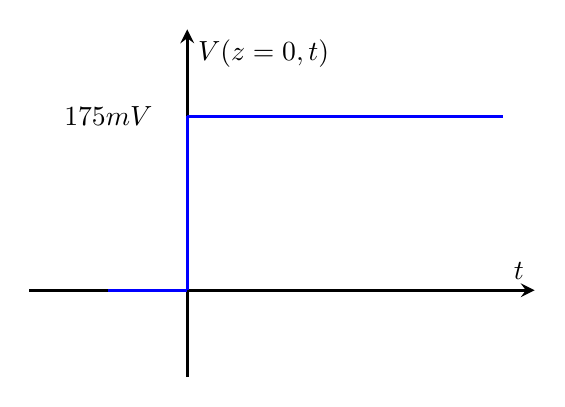
\begin{tikzpicture} 
\begin{axis}[very thick,
                     samples = 100,
                     ytick={-2,2},
                     xlabel = {$t$},
                     ylabel = {$V(z=0, t)$},
                     xmin = -1,
                     xmax = 2.2,
                     ymin = -0.5,
                     ymax = 1.5,
                     width=8cm,
                     height=6cm,
                     axis x line = middle,
                     axis y line = middle,
                     ticks = none]
                     
            \addplot[blue] coordinates {(-0.5,0) (0,0)};
            \addplot[blue] coordinates {(0,0) (0,1)};
            \addplot[blue] coordinates {(0,1) (2,1)};
            \node at (axis cs:-0.5,1){$175 mV$};
            
        \end{axis}
\end{tikzpicture}

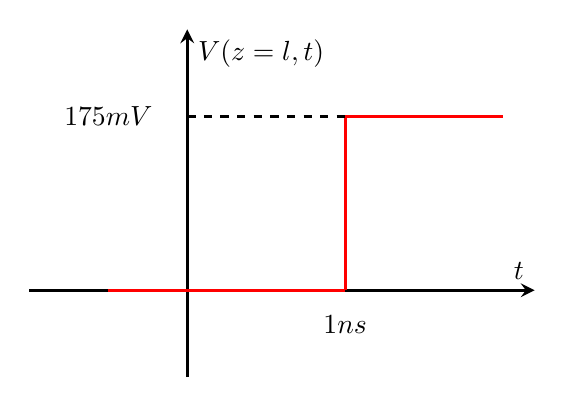
\begin{tikzpicture} 
\begin{axis}[very thick,
                     samples = 100,
                     ytick={-2,2},
                     xlabel = {$t$},
                     ylabel = {$V(z=l, t)$},
                     xmin = -1,
                     xmax = 2.2,
                     ymin = -0.5,
                     ymax = 1.5,
                     width=8cm,
                     height=6cm,
                     axis x line = middle,
                     axis y line = middle,
                     ticks = none]
                     
            \addplot[red] coordinates {(-0.5,0) (1,0)};
            \addplot[red] coordinates {(1,0) (1,1)};
            \addplot[red] coordinates {(1,1) (2,1)};
            \addplot[dashed] coordinates {(0,1) (1,1)};
            \node at (axis cs:-0.5,1){$175 mV$};
            \node at (axis cs:1,-0.2){$1ns$};
            
        \end{axis}
\end{tikzpicture}

\caption{First graph shows the voltage at the start of the line and the second shows the voltage at the end of the line. Source: own.}
\label{graph:1} 
\end{figure}
    
    Como a resposta ao impulso para o filtro casado é dado por: $h(t) = s(T-t)$, tem-se que a representação gráfica é dada pela figura \ref{graph:2} e a sua representação matemática será:
    
    \begin{center}
        $h(t) = \frac{A}{2}[u(T-t) - 2u(T/2-t)] - u(-t)]$
    \end{center}
    
    
\begin{figure}[H]
\centering
\tikz \node [scale=0.8, inner sep=0] {
\begin{tikzpicture} 
    \draw[black, very thick] (-2,3) -- (0,3);
    \draw[black, very thick] (0,3) -- (0,0);
    \draw[black, very thick] (0,0) -- (2,0);
    \node[blue] at (-2.4,3) {$R_{in}$};  
    \node[red] at (2.4,0) {$R_{L}$};  
    \node[black] at (1,1.5) {$1+Q_s^2$};  
    \draw[>=latex, <->] (0.2,0) -- (0.2,3);
    \node[black] at (0,-0.5) {(a)};
\end{tikzpicture}
};
\hspace{1cm}
\tikz \node [scale=0.8, inner sep=0] {
\begin{tikzpicture} [american]
    \draw[>=triangle 90, ->] (-0.5,0) -- (0.5,0);
    \draw[>=triangle 90, ->] (6.5,0) -- (5.5,0);
    \node[black] at (-0.9,0) {$R_{in}$}; 
    \node[black] at (6.9,0) {$R_L$}; 
    \node[black] at (3,-4) {(b)};
    \draw (1,0) to[L, l=$L$, *-*] (5,0)
    (2,0) to[C, l=$C$, *-] (2,-3) node[ground]{}
    ;
\end{tikzpicture}
};

\caption{(a) Desired effect of impedance gain(b) L matching network for a serial to parallel transformation of load impedance. Source: own.}
\label{graph:2} 
\end{figure}
    
    \item Enquanto isso a saída do filtro casado é dada pela convolução entre o sinal de entrada e o filtro, de forma que: $r(t) = s(t) \ast h(t)$. Apesar da tarefa ser exaustiva, a convolução será calculada por partes levando em consideração a representação gráfica. Sendo assim:
    
    \begin{center}
        $0 \leq t \leq T/2$: $r(t) = -\frac{A^2}{4}t$ \\ \vspace{2pt}
        $T/2 < t \leq T$: $r(t) = -\frac{A^2T}{8} + \frac{3A^2}{4}(t-T/2)$ \\ \vspace{2pt}
        $T < t \leq 3T/2$: $r(t) = \frac{A^2T}{4} - \frac{3A^2}{4}(t-T)$ \\ \vspace{1pt}
        $3T/2 < t \leq 2T$: $r(t) = -\frac{A^2T}{8} + \frac{A^2}{4}(t-3T/2)$ \\ \vspace{1pt}
    \end{center}
    
    
\begin{figure}[H]
\centering
\tikz \node [scale=0.8, inner sep=0] {
\begin{tikzpicture} 
    \draw[black, very thick] (-2,1) -- (0,1);
    \draw[black, very thick] (0,1) -- (0,3);
    \draw[black, very thick] (0,3) -- (2,3);
    \draw[black, very thick] (2,3) -- (2,-1);
    \draw[black, very thick] (2,-1) -- (4,-1);
    \node[blue] at (-2.4,1) {$R_{in}$};  
    \node[red] at (4.4,-1) {$R_{L}$}; 
    \node[black] at (1,3.4) {$R_{i}$}; 
    \node[black] at (-1.2,2) {$1+Q_2^2$}; 
    \node[black] at (3.2,1) {$1+Q_1^2$}; 
    \draw[>=latex, <->] (-0.2,1) -- (-0.2,3);
    \draw[>=latex, <->] (2.2,-1) -- (2.2,3);
    \node[black] at (0,-1.5) {(a)};
\end{tikzpicture}
};
\hspace{1cm}
\tikz \node [scale=0.8, inner sep=0] {
\begin{tikzpicture} [american]
    \draw[>=triangle 90, ->] (-2.5,0) -- (-1.5,0);
    \draw[>=triangle 90, ->] (6.5,0) -- (5.5,0);
    \draw[] (2,0.3) -- (2,0.8);
    \draw[>=triangle 90, ->] (2,0.3) -- (2.5,0.3);
    \node[black] at (2,1.2) {$R_{i}$}; 
    \node[black] at (-2.9,0) {$R_{in}$}; 
    \node[black] at (6.9,0) {$R_L$}; 
    \node[black] at (2,-4) {(b)};
    \draw (2,0) to[L, l=$L_1$, *-*] (5,0)
    (2,0) to[C, l=$C$, *-] (2,-3) node[ground]{}
    (-1,0) to[L, l=$L_2$, *-*] (2,0)
    ;
\end{tikzpicture}
};

\caption{(a) Desired effect of impedance gain(b) T matching network for a serial to parallel transformation of load impedance. Source: own.}
\label{graph:3} 
\end{figure}
    
    \item O valor máximo pode ser facilmente encontrado pelo gráfico \ref{graph:3} ou pela expressão matemática como $\frac{A^2T}{4}$ em $t=T$, ou seja, com pico em um instante de amostragem igual ao tempo de símbolo.
\end{subquestion}

\newpage